\documentclass[../main/thesis.tex]{subfiles}
\begin{document}

\chapter{IDE1180 Shape Graphs}
\label{a-shape}

\begin{figure} [h!]%2016.07.18 & 2016.08.12
	\centering
	\begin{subfigure}{.5\textwidth}
		\centering
		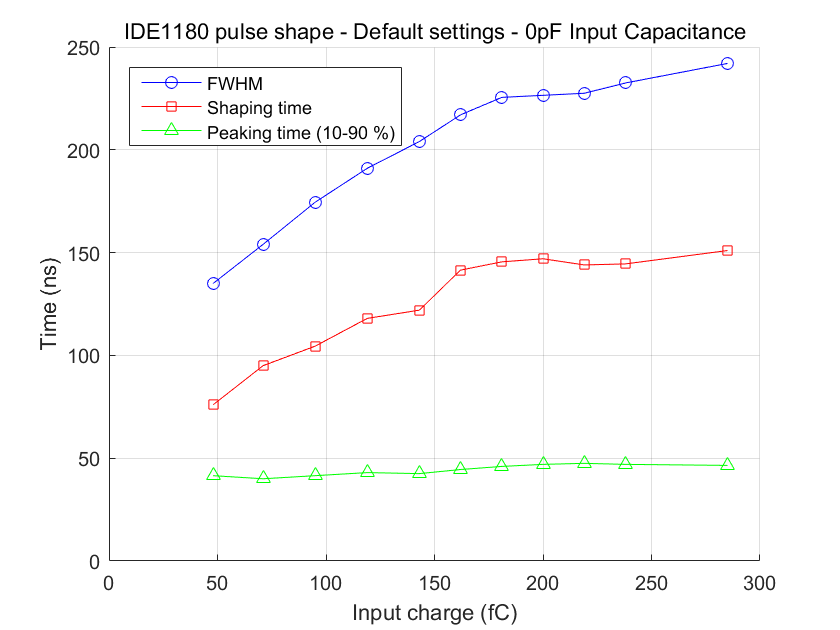
\includegraphics[width=\linewidth]{sh_40_0.png}
		\caption{0 pF input load capacitance.}
		\label{fig-shape-40-0}
	\end{subfigure}%
	\begin{subfigure}{.5\textwidth}
		\centering
		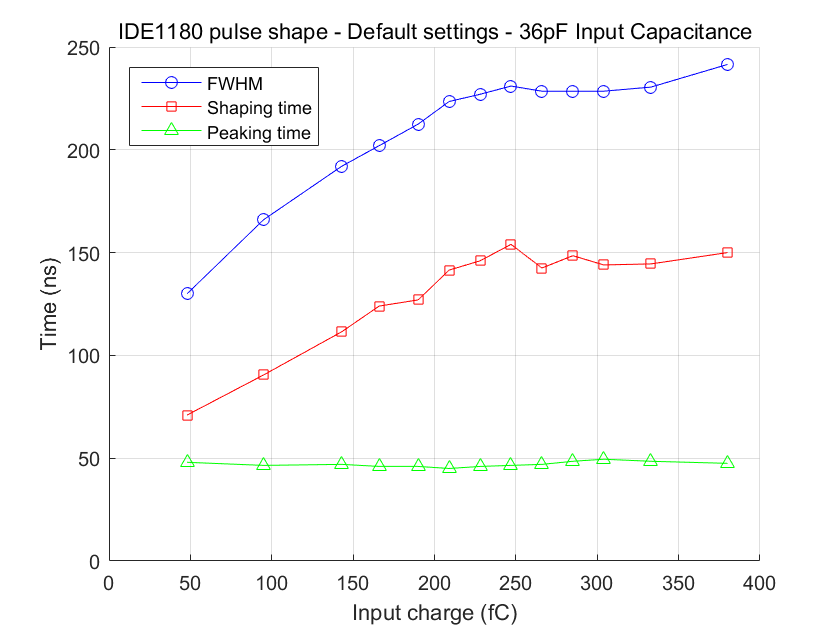
\includegraphics[width=\textwidth]{sh_40_33.png}
		\caption{36 pF input load capacitance.}
		\label{fig-shape-40-33} 
	\end{subfigure}
	\caption{Pulse shape parameters for default settings.}
	\label{fig-shape-def}
\end{figure}

\begin{figure} [h!]%2016.07.18 & 2016.08.12
	\centering
	\begin{subfigure}{.5\textwidth}
		\centering
		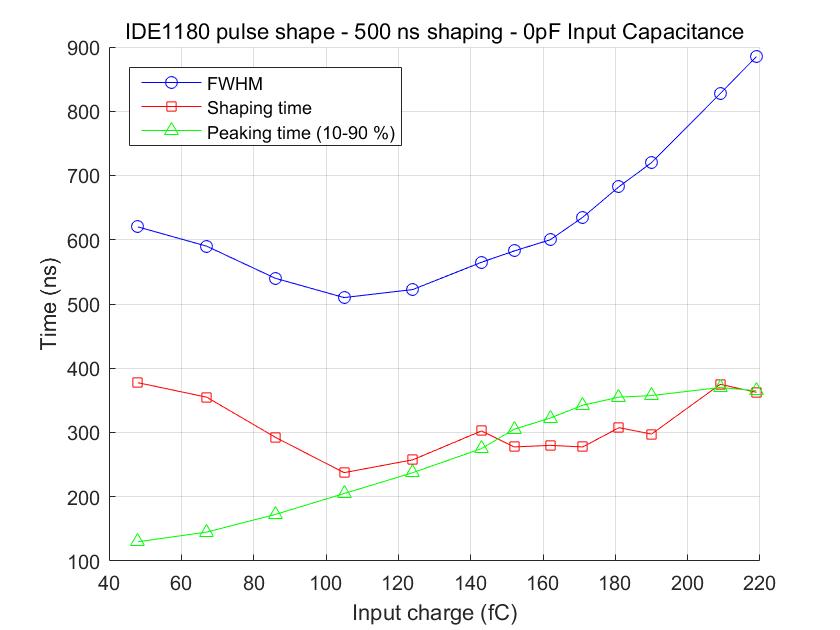
\includegraphics[width=\linewidth]{sh_500_0.png}
		\caption{0 pF input load capacitance.}
		\label{fig-shape-500-0}
	\end{subfigure}%
	\begin{subfigure}{.5\textwidth}
		\centering
		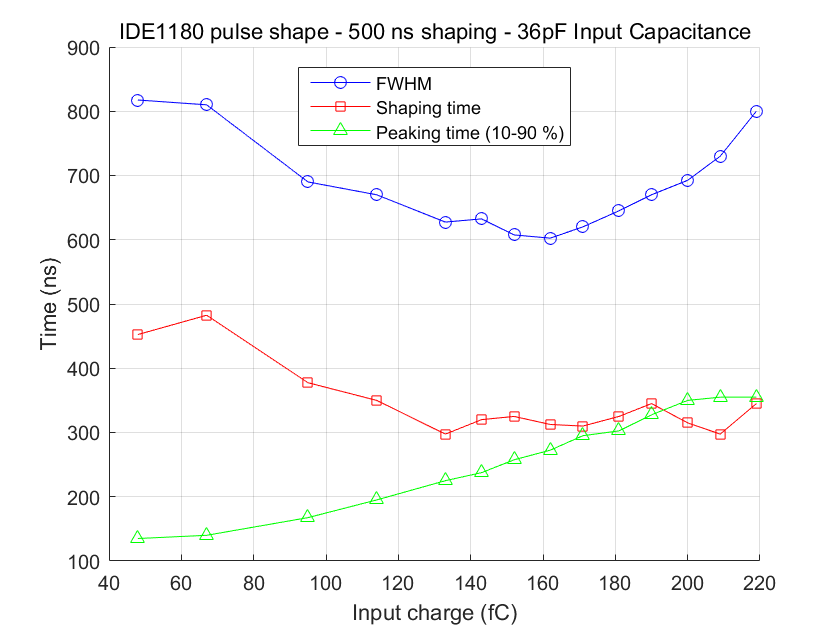
\includegraphics[width=\textwidth]{sh_500_33.png}
		\caption{36 pF input load capacitance.}
		\label{fig-shape-500-33} 
	\end{subfigure}
	\caption{Pulse shape parameters for 500 ns shaping time.}
	\label{fig-shape-500}
\end{figure}

\begin{figure} %2016.07.18 & 2016.08.12
	\centering
	\begin{subfigure}{.5\textwidth}
		\centering
		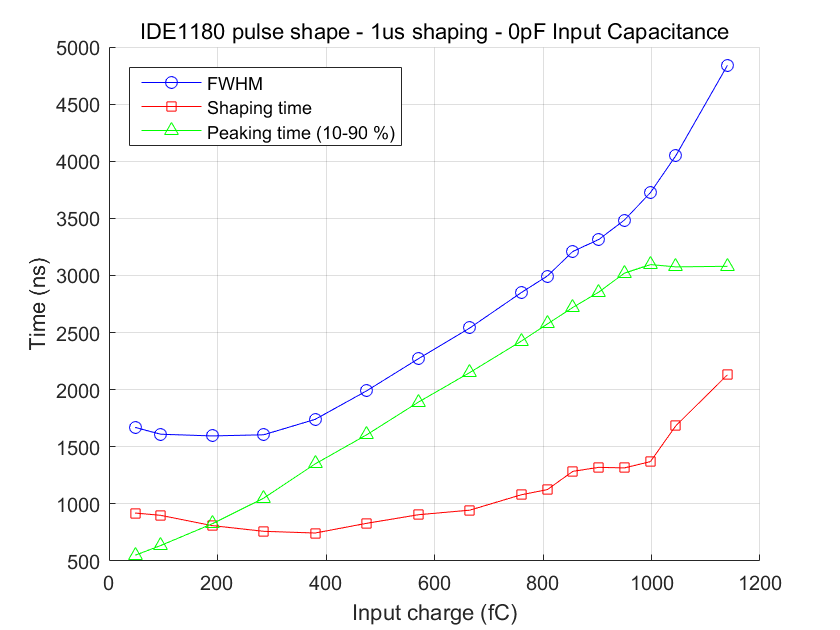
\includegraphics[width=\linewidth]{sh_1_0.png}
		\caption{0 pF input load capacitance.}
		\label{fig-shape-1-0}
	\end{subfigure}%
	\begin{subfigure}{.5\textwidth}
		\centering
		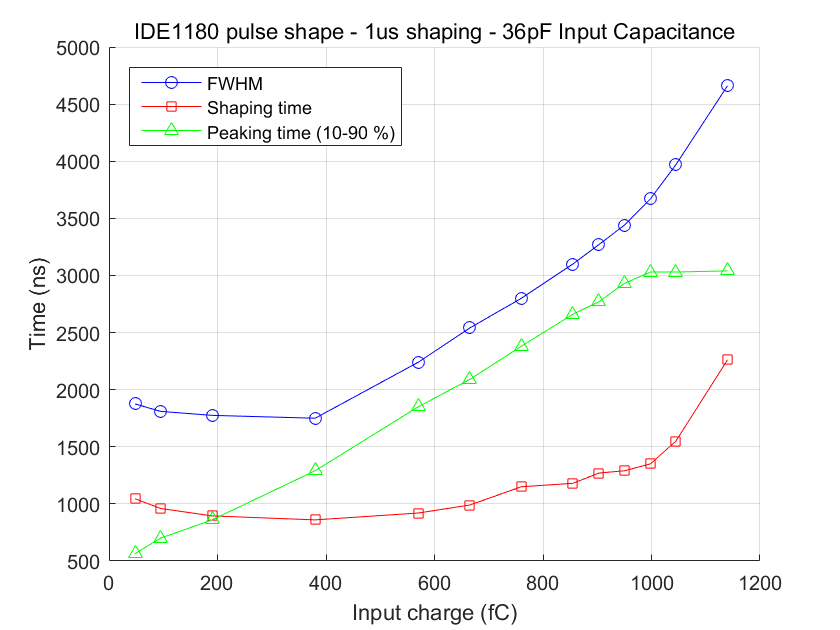
\includegraphics[width=\textwidth]{sh_1_33.png}
		\caption{36 pF input load capacitance.}
		\label{fig-shape-1-33} 
	\end{subfigure}
	\caption{Pulse shape parameters for 1 $\mu$s shaping time.}
	\label{fig-shape-1}
\end{figure}

\begin{figure} %2016.07.18 & 2016.08.12
	\centering
	\begin{subfigure}{.5\textwidth}
		\centering
		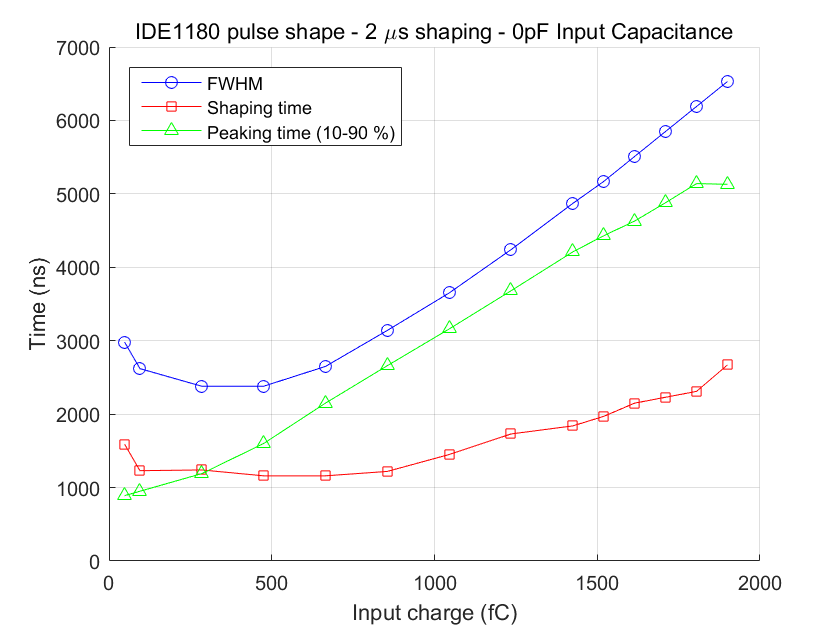
\includegraphics[width=\linewidth]{sh_2_0.png}
		\caption{0 pF input load capacitance.}
		\label{fig-shape-2-0}
	\end{subfigure}%
	\begin{subfigure}{.5\textwidth}
		\centering
		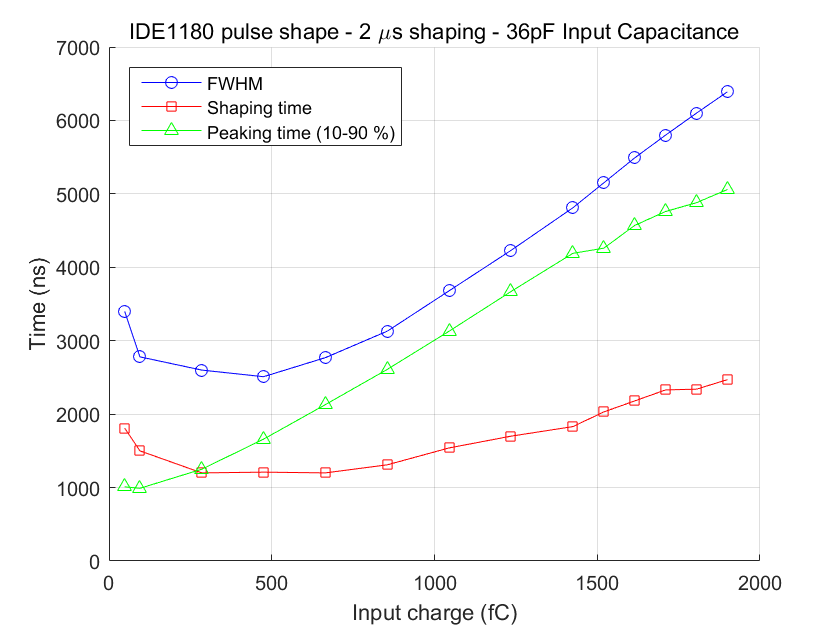
\includegraphics[width=\textwidth]{sh_2_33.png}
		\caption{36 pF input load capacitance.}
		\label{fig-shape-2-33} 
	\end{subfigure}
	\caption{Pulse shape parameters for 2 $\mu$s shaping time.}
	\label{fig-shape-2}
\end{figure}

\end{document}